\chapter{Targeted Proteolysis}
\label{chap:tarprot}

The module Targeted Proteolysis is designed to post-process the mass spectrometry
data acquired during the enzymatic proteolysis of a Target protein by a single
protease. In a typical experimental setup both the protease and the Target protein
are mixed together under various experimental conditions and the peptides generated
during the proteolysis are identified by mass spectrometry. It is expected that
several control experiments and several replicates of the tested experimental
conditions are performed. The main objective of the module is to identify the peptides
with intensity values that are significantly different in the control experiments
and the replicates of the various experimental condition tested at the chosen
significance level.

\section{Definitions}

Before explaining in detail the interface and how does the module work, let's make
clear the meaning of the term Filtered peptide in the context of the Targeted 
proteolysis module:

\phantomsection
\begin{itemize}
    \item \textit{Filtered peptide}: a relevant peptide with a significantly different
    behavior in the control and a given experiment at the chosen significance level.
    \label{par:tarprotPIP}
\end{itemize}

The rest of the definitions in \autoref{sec:limprotDefinitions} are valid for this
module too.

\section{The input files}

The Targeted Proteolysis module requires a Data file containing the detected peptides
and a sequence file containing the amino acid sequence of the recombinant protein
used in the study. Both files must follow the guidelines specified in \autoref{sec:dataFile}.
In short, the Data file must have a tabular format with tab separated columns and
the name of the columns are expected as first row. The Sequence file is expected
to contain at least one sequence and to be FASTA formatted. If more than one sequence
is found in the Sequence file the first sequence will be taken as the sequence of
the Recombinant protein and the second sequence will be taken as the sequence of
the Native protein. All other sequences are discarded.

\section{The interface}

The tab of the Targeted Proteolysis module is divided in two regions (\autoref{fig:tarprotTab}).

\begin{figure}[h]
    \centering
    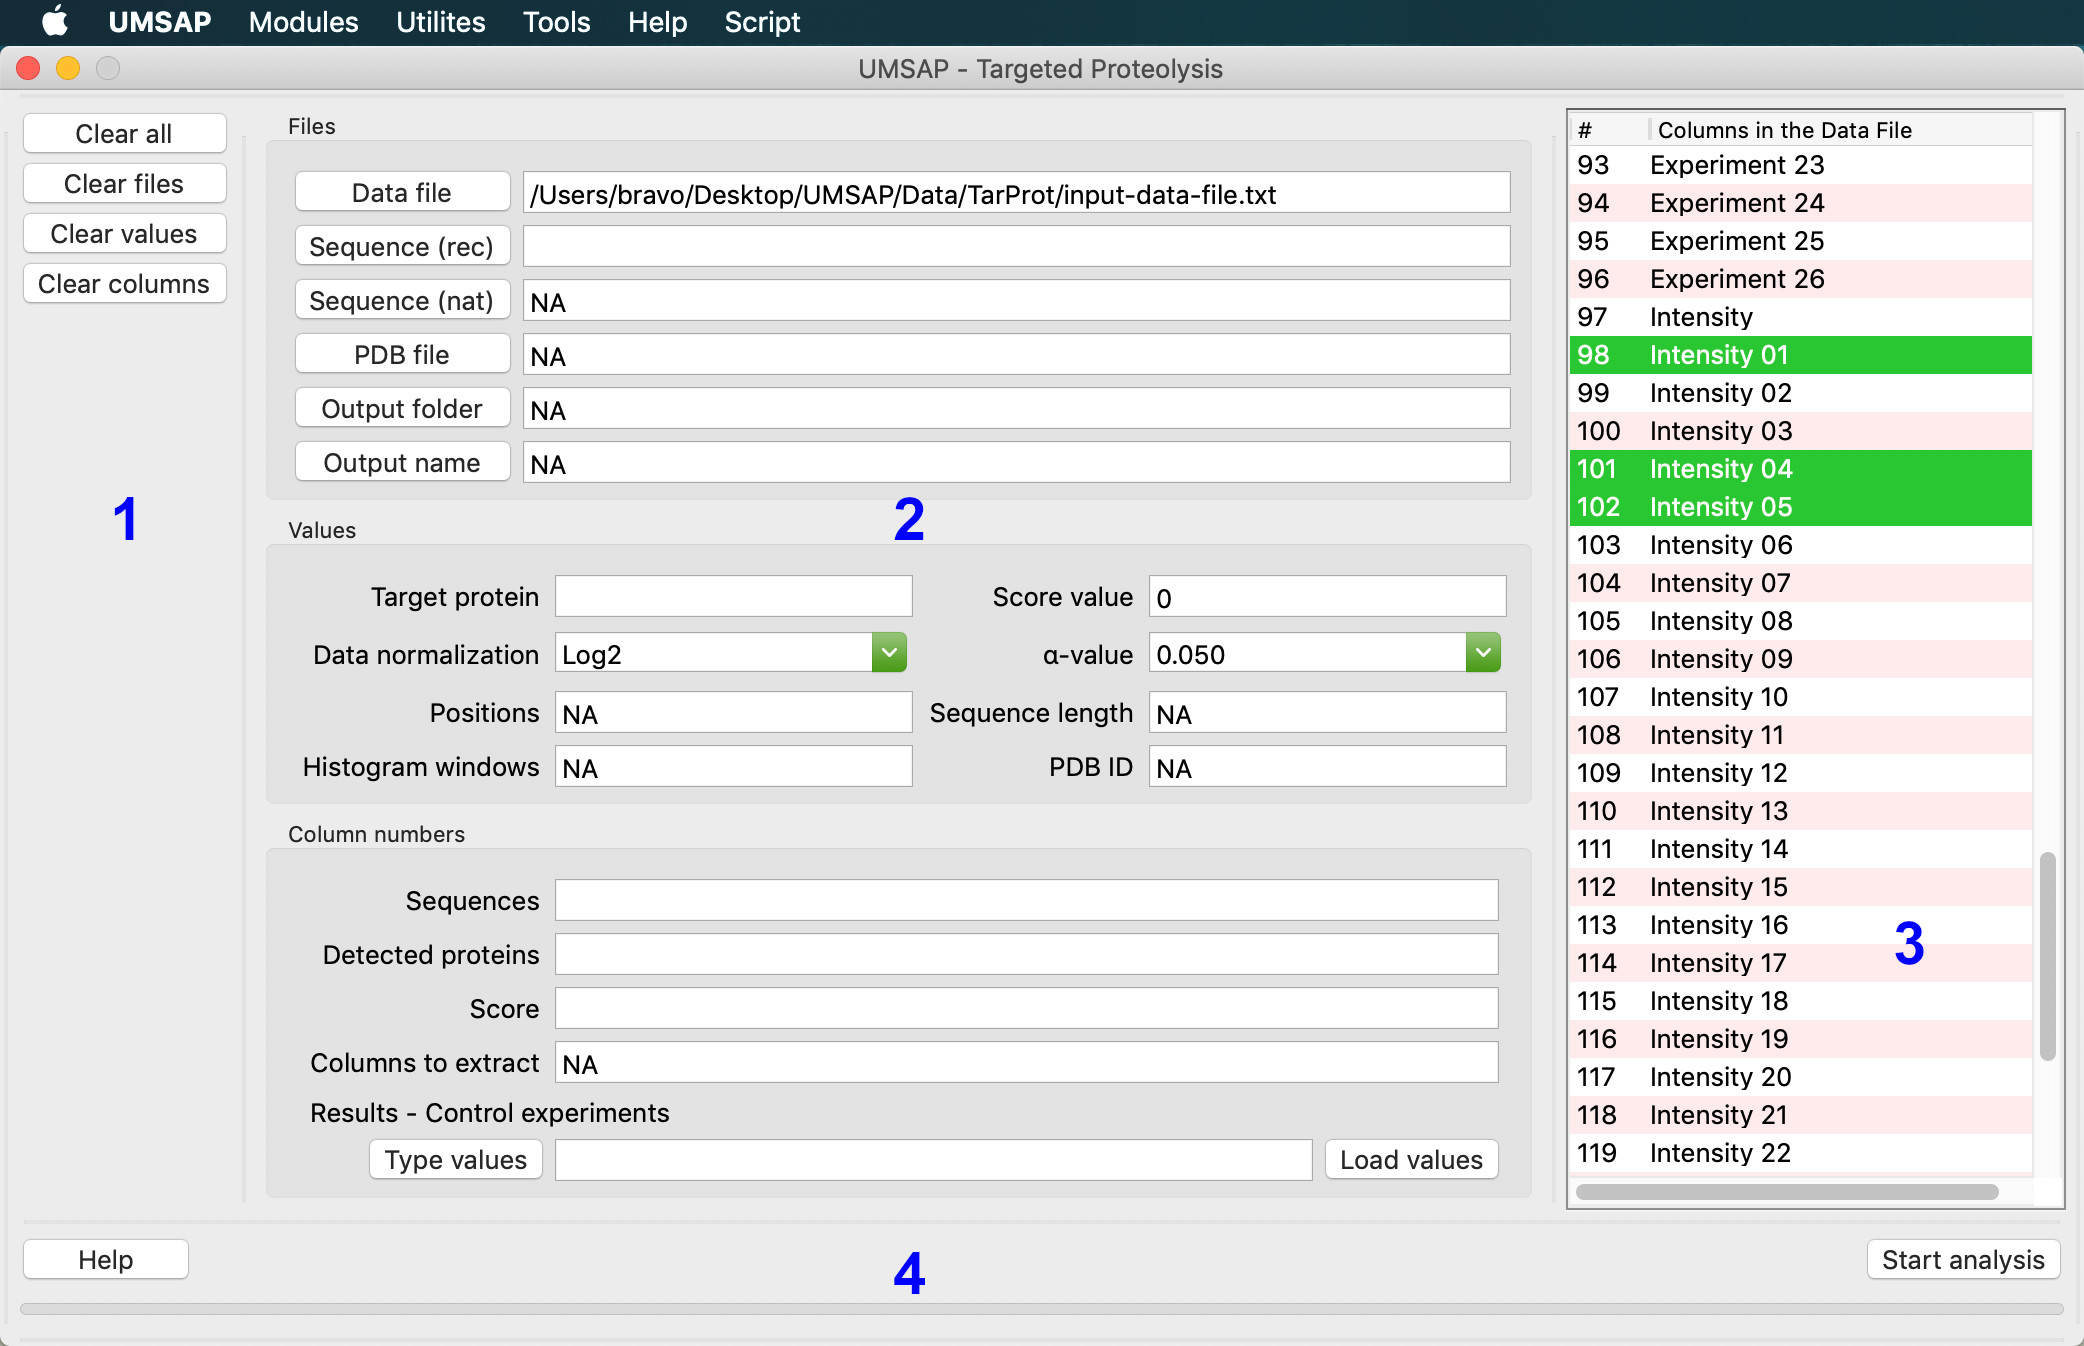
\includegraphics[width=0.7\textwidth]{./IMAGES/MOD-TARPROT/tarprot-mod.jpg}
    \caption[The Targeted Proteolysis module tab]{\textbf{The Targeted Proteolysis
    module tab.} This tab allows users to perform the analysis of the results obtained
    during an enzymatic proteolysis experiment.}
    \label{fig:tarprotTab}
    \vspace{-5pt}
\end{figure} 

The Data File Content region holds only a table to show the name of the columns in
the selected Data File. The table will be automatically filled after selecting the
file. Selected rows in the table can be copied (Cmd+C) and pasted (Cmd+V) to the
text fields in region Configuration Options.

The Configuration Options region contains all the fields needed to configure and
run the analysis.

Section Files contains three buttons and a text field. Here users select the input
and output files for the analysis.

\num{1}. The button UMSAP allows users to browse the file system to select the location
and name of the .umsap file. When selecting an already existing .umsap file the operating
system will ask if it is ok to replace the file, the answer can be yes since UMSAP
will never overwrite or replace an .umsap file, instead the new analysis will be
added to the already existing file. Only .umsap files can be selected here.

\num{2}. The button Data allows users to browse the file system to select the input
data file that will be used for the analysis. The Data file is expected to be a
plain text file with tab separated columns and the name of the columns in the first
row of the file. In addition, columns to be analyzed must contain only numbers and
must be of the same length. Only .txt files can be selected here.

\num{3}. The button Sequences allows users to browse the file system to select the
FASTA file containing the sequence of the Recombinant protein and the Native protein.
The FASTA file must contain at least one sequence.

\num{4}. The text field Analysis ID allows users to provide an ID for the analysis
to be run. The date and time of the analysis will be automatically added to the
beginning of the name.

Section Data Preparation contains four dropdown boxes. Here users select how the data
in the Data file should be prepared before starting the analysis.

\num{1}. The dropdown Treat \num{0}s as missing values allows user to define how
to handle \num{0} values present in the Data file.

\num{2}. The dropdown Transformation allows user to select the Transformation method
to be applied to the data.

\num{3}. The dropdown Normalization allows users to select the Normalization method
to be applied to the data.

\num{4}. The dropdown Imputation allows user to select the Imputation method used
to replace missing values in the data.

Section User-defined values contains five text fields Here users configure the 
Targeted Proteolysis analysis to be run.

\phantomsection
\num{1}. The text field Target Protein\label{par:limprotTargetProtein} allows users
to specify the protein of interest. Users may type here any unique protein identifier
present in the Data file. The search for the Target Protein is case-sensitive, meaning
that eFeB is not the same as efeb.

\phantomsection
\num{2}. The text field Score Value\label{par:limprotScoreValue} allows users to
define a threshold value above which the detected peptides will be considered as
relevant. The Score Value is an indicator of how reliable was the detection of the peptide
during the MS experiments. The value given to UMSAP depends on the program generating
the Data file. Only one real number equal or greater than zero will be accepted here.
A value of zero means all detected peptides belonging to the Target Protein will
be treated as relevant peptides.

\num{3}. The text field $\alpha$ level allows users to define the significance level
used for the analysis. Only a number between \num{0} and \num{1} will be accepted
here.

\phantomsection
\num{4}. The text field AA Positions\label{par:tarprotPos} allows users to define
the number of positions to be considered during the amino acid (AA) distribution
calculation (\autoref{subsec:tarprotAA}). Only one integer number greater than zero
will be accepted here. If left empty the calculation will not be performed.

\phantomsection
\num{5}. The text field Histogram Windows\label{par:tarprotHist} allows users to
define the size of the windows for the Histogram analysis (\autoref{subsec:tarprotHist}).
Only integer numbers equal or greater than zero will be accepted here. In addition,
the values must be organized from smaller to bigger values. Users may specify a fix
histogram window size by given just one integer number greater than zero. In this
case the histogram will have even spaced windows with the width specified by Histogram
Windows. If more than one number is provided here, then windows with the customs width
will be created. For example, the input \numlist{50 100} will create only one window
including cleavage sites between residues \numrange{50}{99}. The input
\numlist{1 50 100 150} will create three windows including cleavages sites between
residues \numrange{1}{49}, \numrange{50}{99} and \numrange{100}{149}. Duplicate values
are not allowed. If left empty the histogram will not be created.

Section Column numbers contains four text fields. Here, users provide the column
numbers in the Data file from where UMSAP will get the information needed to perform
the analysis of the module. All columns specified in this section must be present
in the Data file. Column numbers start at \num{0}. The column numbers are shown in
the table of Region Data File Content after the Data file is selected.

\num{1}. The text field Sequences allows users to specify the column in the Data
file containing the sequences of the peptides identified in the MS experiments.
Only one integer number equal or greater than zero will be accepted here.

\num{2}. The text field Detected Proteins allows users to specify the column in
the Data file containing the unique protein identifier for the proteins detected
in the MS experiments. It is in this column where the program will look for the
Target Protein value given in Section User-defined values. It is important that
in this column the Target Protein value is used to refer to only one protein. Only
one integer number equal or greater than zero will be accepted here.

\num{3}. The text field Score allows users to specify the column in the Data file
containing the Score values. It is in this column where the program will look for
the values to be compared against the Score threshold given in Section User-defined
values.

\phantomsection
\num{4}. \label{par:limprotResultControl}The text field Results - Control experiments
allows users to specify the columns in the Data file containing the results of the
control and experiments. The button Type Values call a helper window
(\autoref{fig:tarprotResControlWindow}) where users can type the information needed. 

\begin{figure}[h]
    \centering
    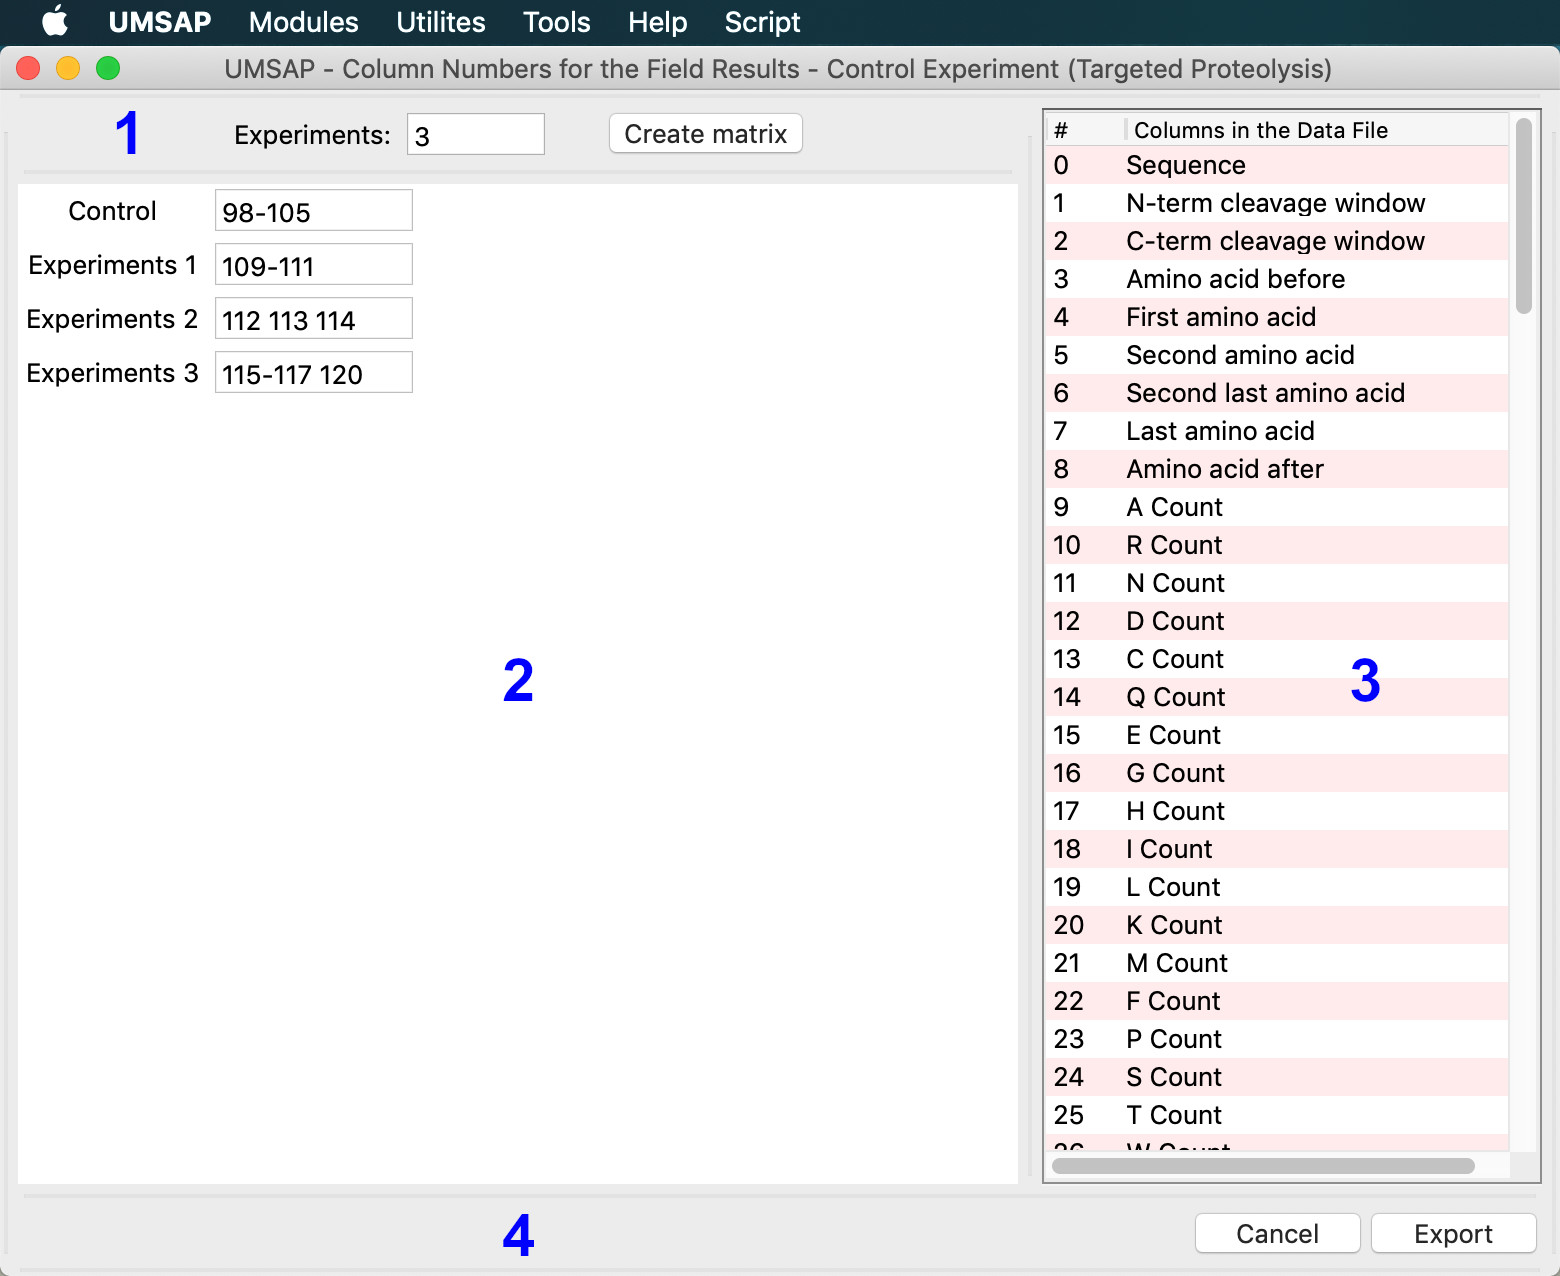
\includegraphics[width=0.7\textwidth]{./IMAGES/MOD-TARPROT/tarprot-rescontrol.jpg}
    \caption[The Result - Control experiments helper window for the Targeted Proteolysis module]{\textbf{The Result - Control experiments helper window for the Targeted Proteolysis module.} This window allows users to specify the column numbers in the Data file containing the MS results for the selected experiments and control.} 
    \label{fig:tarprotResControlWindow}
    \vspace{-5pt} 	
\end{figure}

The helper window is divided in two Regions. Region Data File Content will show the 
column numbers and names of the columns present in the selected Data file. Region
Configuration Options has two sections. The upper section allows defining the number
of experiments performed as well as the label for the control and experiments. The
button Setup Fields creates the corresponding text fields in the bottom section to
type the column numbers. Each text field should contain the column numbers with the
MS results for the given experiment. The values for the text fields should be positive
integer numbers or a range of integers, e.g. \numrange[range-phrase=--]{60}{62}.
Selected rows in the table can be copied (Cmd+C) and then pasted (Cmd+V) in the text
fields. Duplicate column numbers are not allowed.

\section{The analysis}

First, UMSAP will check the validity of the user-provided input and then the selected
Data file is read. The columns specified in section Column numbers are extracted
from the Data file. All other columns present in the Data file are discarded. After
this, all steps selected in the Data Preparation section are applied to the columns
specified in the text field Result - Control experiments (\autoref{chap:dataPrep}).
Then, the following actions are performed.

All rows in the Data file containing peptides that do not belong to the Target protein
are removed. Then, all rows containing peptides from the Target protein but with
Scores values lower than the user-defined Score threshold are removed. These steps
leave only relevant peptides, this means peptides with a Score value higher than
the user defined threshold that belong to the Target protein. For each one of these
relevant peptides a test for Homogeneity of Regression \cite{ancova} is performed.

\phantomsection
The test, \label{par:tarprotAncovaTest} done to identify relevant peptides with
different intensities in the control and a given experiment, is performed in three
steps. First, the intensity values for the replicates in the control and in a given
experiment are organized in two data sets as indicated in \autoref{fig:tarprotAncova}.
Each data set consist of two points. For the control data set the intensity values
in the replicates of the control experiment are allocated to both points. For the
experiment data set the intensity of the replicates in the control experiment are
allocated to the first point and the intensity values of the replicates in the given
experiment are allocated to the second point. The second step is to find the slope
of the straight line best fitting each data set. The third step is to test the
Homogeneity of Regression. Peptides that fail this test are included in the list of
filtered peptides (FP) because the slopes of the straight lines fitting the data
sets are significantly different at the chosen significance level. The fact that
the slopes are different implies that the peptide is found in an increased
concentration in the given experiment than in the control experiment. Only positive
slopes are considered. Peptides that past this test are not included in the list of
FP for the given experiment. 

\begin{figure}[h]
    \centering
    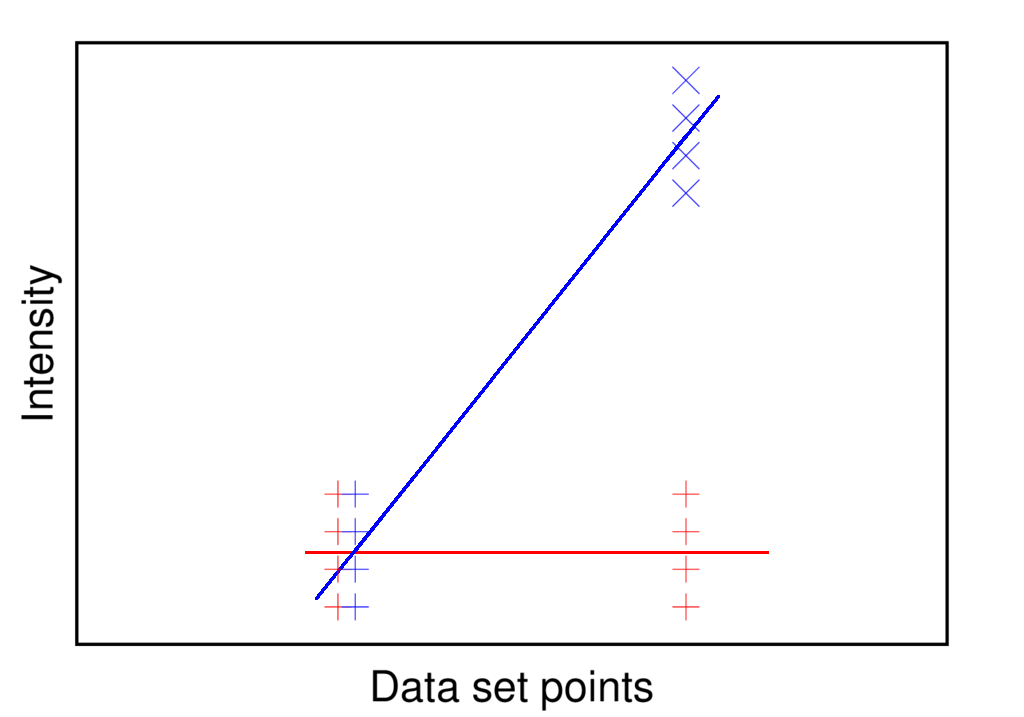
\includegraphics[width=0.7\textwidth]{./IMAGES/MOD-TARPROT/tarprot-ancova.png}	    
    \caption[Data organization prior to the Homogeneity of Regression test]{\textbf{Data
    organization prior to the Homogeneity of Regression test.} Two data sets with
    two points each are created, one data set for the control (red) and one for a
    given experiment (blue). The intensity data in the replicates of the control is
    used in both data points for the control (+) and in the first data point of the
    given experiment. The intensity data in the replicates of the given experiment
    is used for the second point of the data set for the given experiment (x). After
    this, the best fitting line for each data set is found and the slopes of the
    lines are compared in a test for Homogeneity of Regression.} 
    \label{fig:tarprotAncova}
    \vspace{-5pt} 	
\end{figure} 

\section{The result window}

The window showing the results from a Targeted Proteolysis analysis is divided in
four regions (\autoref{fig:tarprotFra}).

\begin{figure}[h]
    \centering
    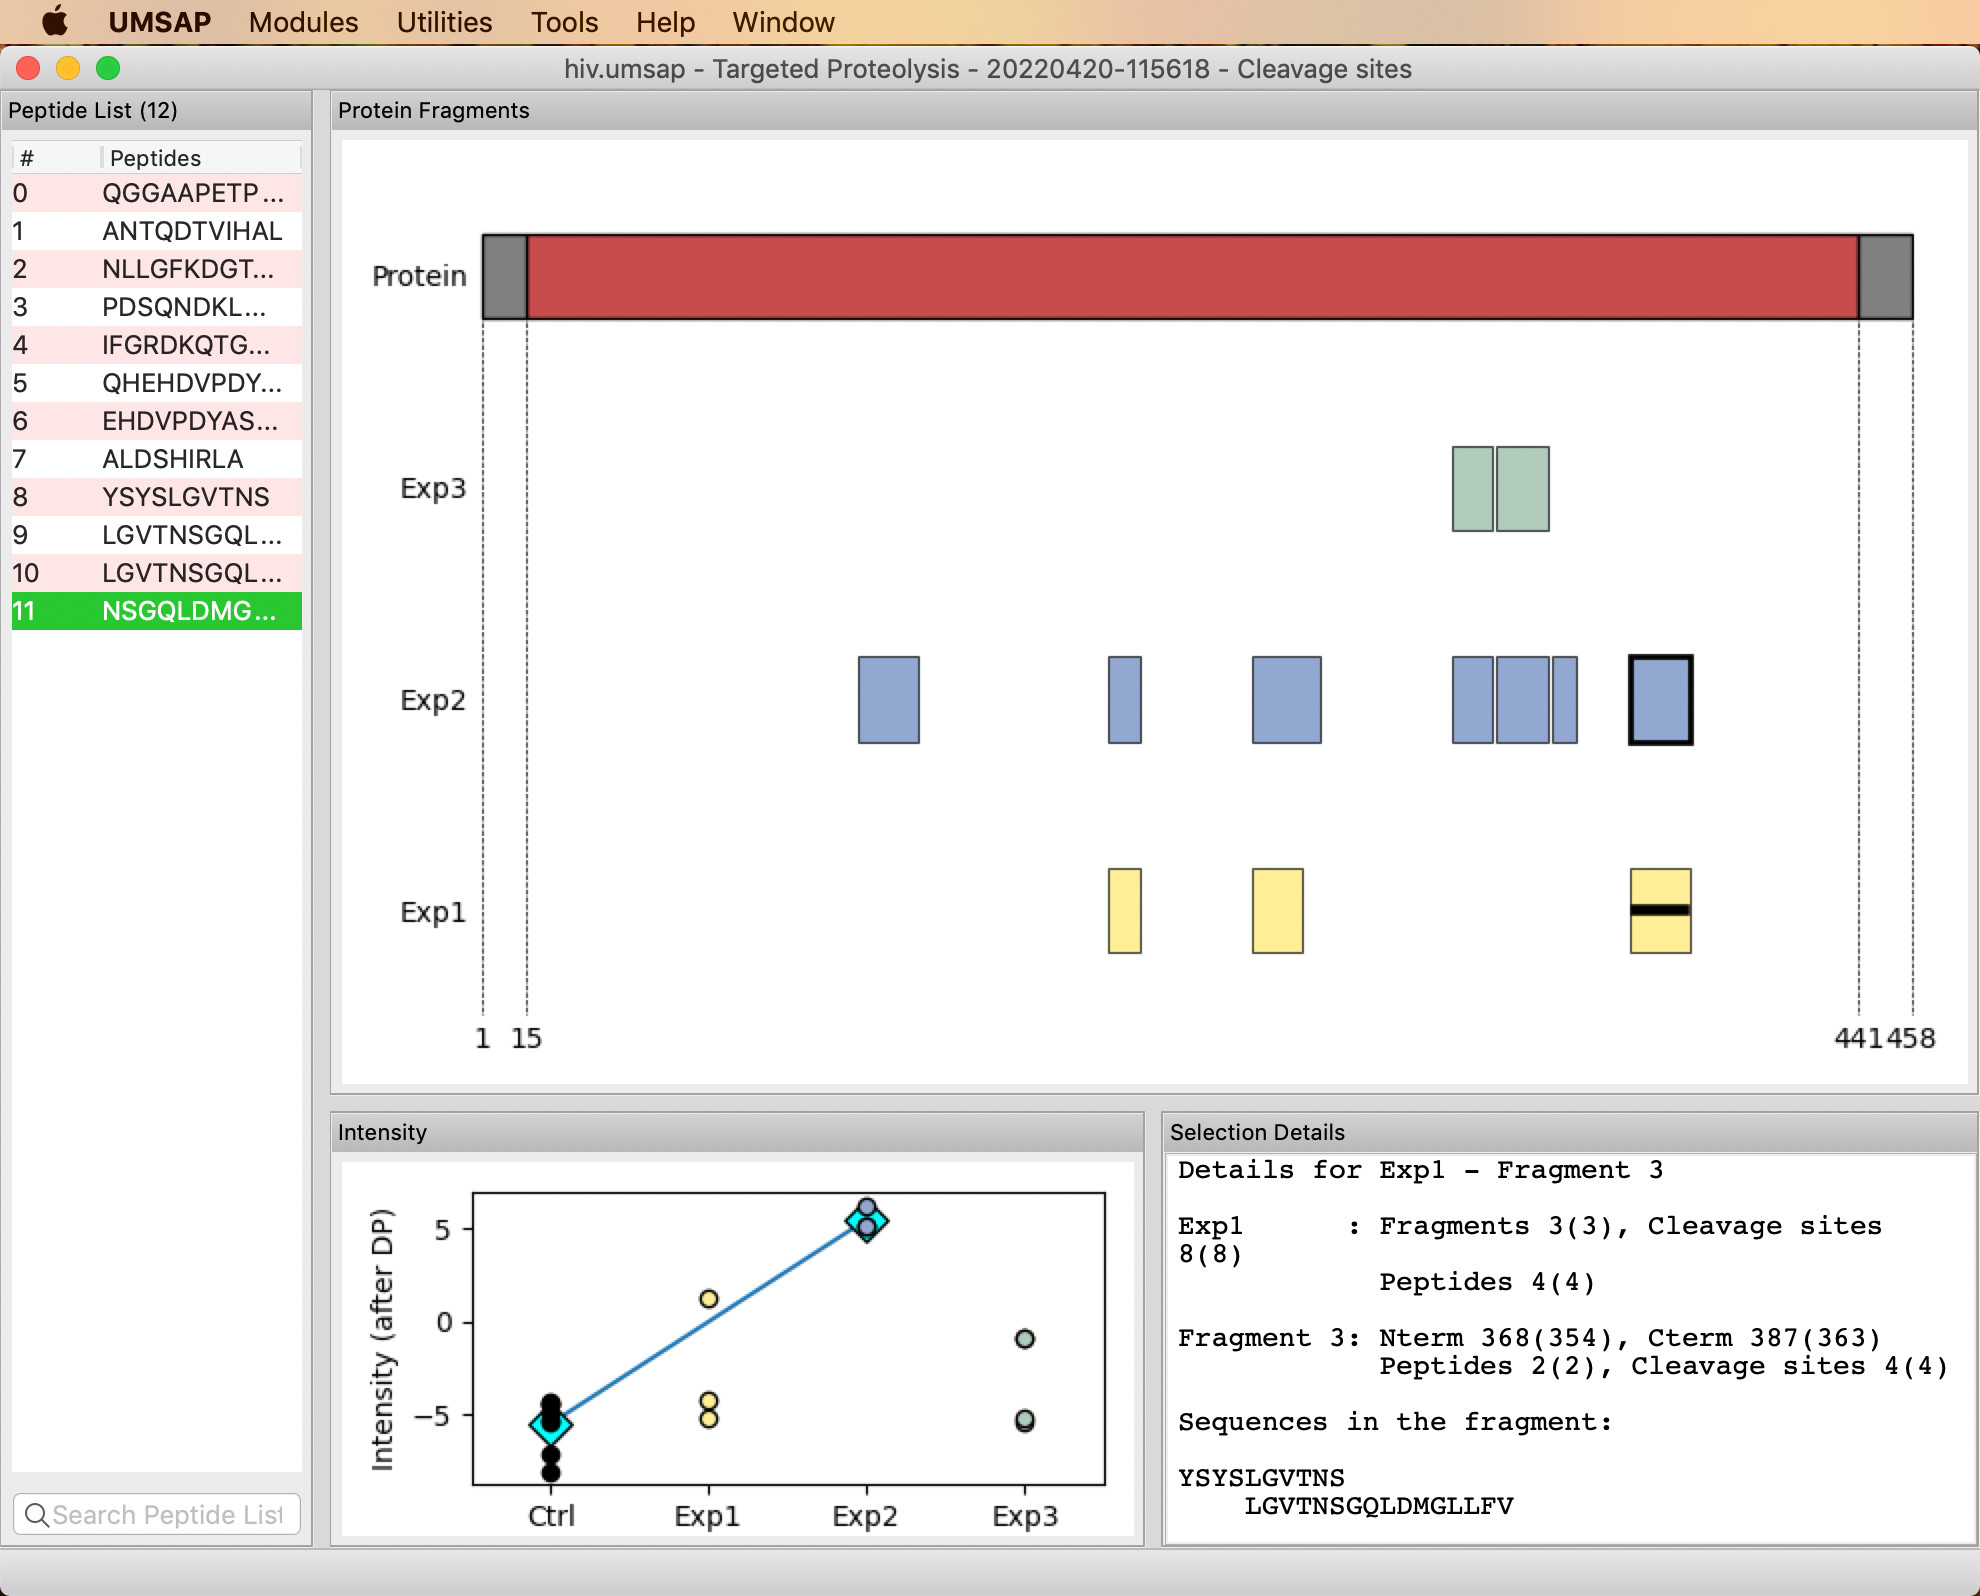
\includegraphics[width=0.8\textwidth]{./IMAGES/MOD-TARPROT/tarprot-frag.jpg}
    \caption[The Fragment analysis window]{\textbf{The Fragment analysis window.}
    Users can perform here the analysis of the fragments obtained in the enzymatic
    proteolysis experiments.}
    \label{fig:tarprotFra}
    \vspace{-5pt}
\end{figure} 

Region Peptide List contains a table with all FP detected during the analysis. Selecting
a peptide in the table will highlight with a thick black border all fragments in
region Protein Fragments where the selected peptide was found. In addition, region
Intensity will show the behavior of the intensity values in the control and experiments
for the selected peptide. The search box at the bottom allows searching for a sequence
in the list of FP.

Region Protein Fragments will display a graphical representation of the fragments
found in each experiment. The first fragment in this region represents the full length
of the recombinant sequence of the Target protein. Here the central red section represents
the sequence in the recombinant protein that is identical to the native protein sequence
while gray sections represent the sequences in the recombinant protein that are different
to the native protein sequence. If the sequence of the native protein was not given
then the fragment is shown in gray. Selecting a fragment will update the information
shown in regions Selection Details.

Region Intensity will display a plot of Intensities vs experiment label. The plot
will display the data for a single peptide selected in the table of region Peptide
List. The intensity values in the plot are the ones obtained after applying the Data
Preparation workflow specified for the analysis. The values for replicates are shown
as circles. The average for a given experiment is shown as bigger cyan diamonds.
The blue lines only connect the control experiment and experiments showing intensity
values significantly different at the chosen significance level.

Region Selection Details will display detailed information about a selected fragment
in Region Protein Fragments. In this Region regular numbers refer to the Recombinant
protein sequence while number between parenthesis refers to the Native sequence.
The Experiment section in the text contain information about the experiment in which
the fragment was identified. The information includes the total number of fragments,
the total number of sequences and the total number of unique cleavage sites identified
in the experiment. The Fragment section in the text gives similar information about
the selected fragment and also includes the first and last residue numbers in the
fragment. The rest of the lines show a sequence alignment of all the peptides in
the fragment.

\section{The Tools menu}

The Tools menu in the window showing the results from a Targeted Proteolysis analysis
allows user to view any of the analyses contained in the selected .umsap file. The
submenus Fragments and Intensities allow resetting the zoom level and create an image
of the corresponding plots.

The submenu Clear Selection allows removing any selection done by the user. In
particular, the entry All (Cmd+K) will remove all selections basically resetting
the state of the window.

The Tools menu also allows duplicating the window (Cmd+D) for easier comparison of
two or more analysis, checking the Data Preparation steps of the analysis (Cmd+P),
exporting the results of the analysis to a tab separated CSV file (Cmd+E) and to
export the sequence alignments (Cmd+S) between the peptides found in the analysis
and the sequence of the recombinant protein. In addition, the zoom level in the plots
can be reset (Shift+Alt+Z) and an image of the plots can be created (Shift+Alt+I).

The submenu Further Analysis give access to other analysis that can be performed
with the information obtained with the Targeted Proteolysis analysis.

\subsection{AA Distribution}
\label{subsec:utilAadistCalc}
The AA Distribution utility allows user to calculate the AA distribution around the detected cleavage sites using a list of FP (see page \pageref{par:tarprotPIP}). The list of FP is automatically generated from a .tarprot file. How to generate a .tarprot file is discussed in \autoref{chap:tarprot}. The list of FP is a non redundant list. 

\textit{\textbf{The interface}}

The window of the AA Distribution utility is divided in three regions (\autoref{fig:utilAadistCalc}).

\begin{figure}[h]
	\centering
	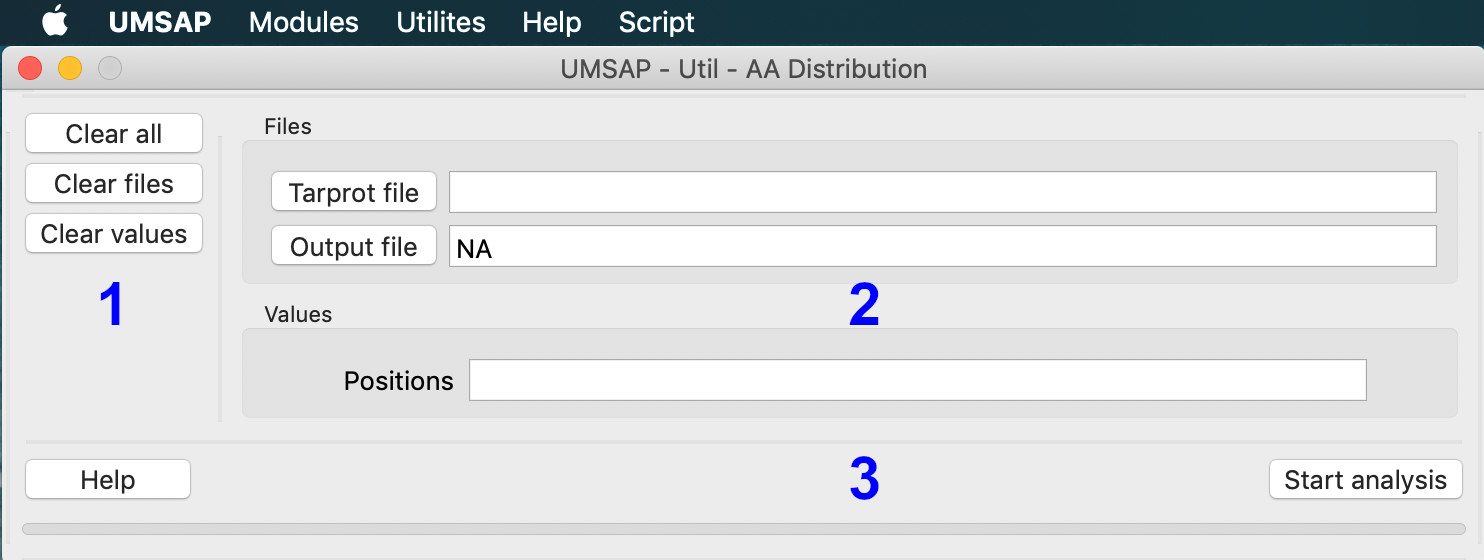
\includegraphics[width=0.7\textwidth]{./IMAGES/UTIL-AA-WINDOW/util-aa.jpg}	    
	\caption[The AA Distribution utility window]{\textbf{The AA Distribution utility window.} This window allows to obtain the AA distribution around the detected cleavage sites from a .tarprot file.} 
	\label{fig:utilAadistCalc}
	\vspace{-5pt} 	
\end{figure}

Region \num{1} contains three buttons allowing users to quickly delete all provided input to generate a new .pdf file. The Clear all button will delete all user provided input. The Clear files button will delete all values in section Files of Region \num{2}. Finally, the Clear values button will delete all values in section Values of Region \num{2}.

Region \num{2} contains the fields where users provide the information needed in order to perform the AA distribution calculation. The Tarprot file button allows users to browse the file system to select the .tarprot file that will be used for the analysis. Only one .tarprot file can be provided here. The Output file button allows users to browse the file system to select the location and name of the Output file. If left empty, then the .aadist file, resulting from the analysis, will be saved in the same directory containing the .tarprot file and will have the same name as the .tarprot file. If the folder containing the selected .tarprot file already contains a .aadist file with the same name as the selected .tarprot file, then UMSAP will add the current date and time to the seconds to the end of the .aadist file in order to avoid overwriting the older .aadist file without explicit user permission.    

The parameter Positions indicates the number of positions around the cleavage sites to be analyzed. The value here must be an integer number greater than zero.

Region \num{3} contains the Help and Start analysis buttons and a progress bar. The Help button leads to an online tutorial while the Start analysis button will start the analysis. The progress bar will give users a rough idea of the remaining processing time once the analysis is started.

\textit{\textbf{The analysis}}

First, UMSAP will check the validity of the user provided input. After this, a list of FP is created using the .tarprot file. For each FP, the sequence around the N and C terminal ends of the peptide is analyzed up to the user provided number of Positions. For the N terminus of the peptide the identity of residues in positions \(Pn\) to \(P1\) is inferred from the sequence of the recombinant protein contained in the .tarprot file. The same is done for positions \(P1'\) to \(Pn'\) at the C terminus of the peptide. If the N or C terminus of a peptide is the first or last residue of the recombinant protein under study the N or C terminus is excluded from the analysis. For each position the number of times that each AA appears at a given position are counted. Finally, the absolute numbers of AA appearances for each position are converted to percent taking the total for each position as the sum of all counted AA in the position.

In addition, UMSAP tests whether the obtained AA distribution is significantly different to the expected AA distribution from the proteolysis of the Target protein by a totally non-selective protease. The first step is to generate an AA distribution with the same number of positions defined by the user with the Position parameter. This distribution is generated assuming that all peptidic bonds in the recombinant protein may be cleaved by the protease with equal probability and that all peptidic bonds will be cleaved. Here, we are also assuming that all products of cleaving all peptidic bonds will be detected in the MS experiment. Then, UMSAP compares each position in both distributions using a $\chi^2$ test with the significance level found in the .tarprot file. In order to be able to perform the $\chi^2$ test, AAs are pooled together in the same groups as described below for the color code used in the output.    

\begin{figure}[h]
	\centering
	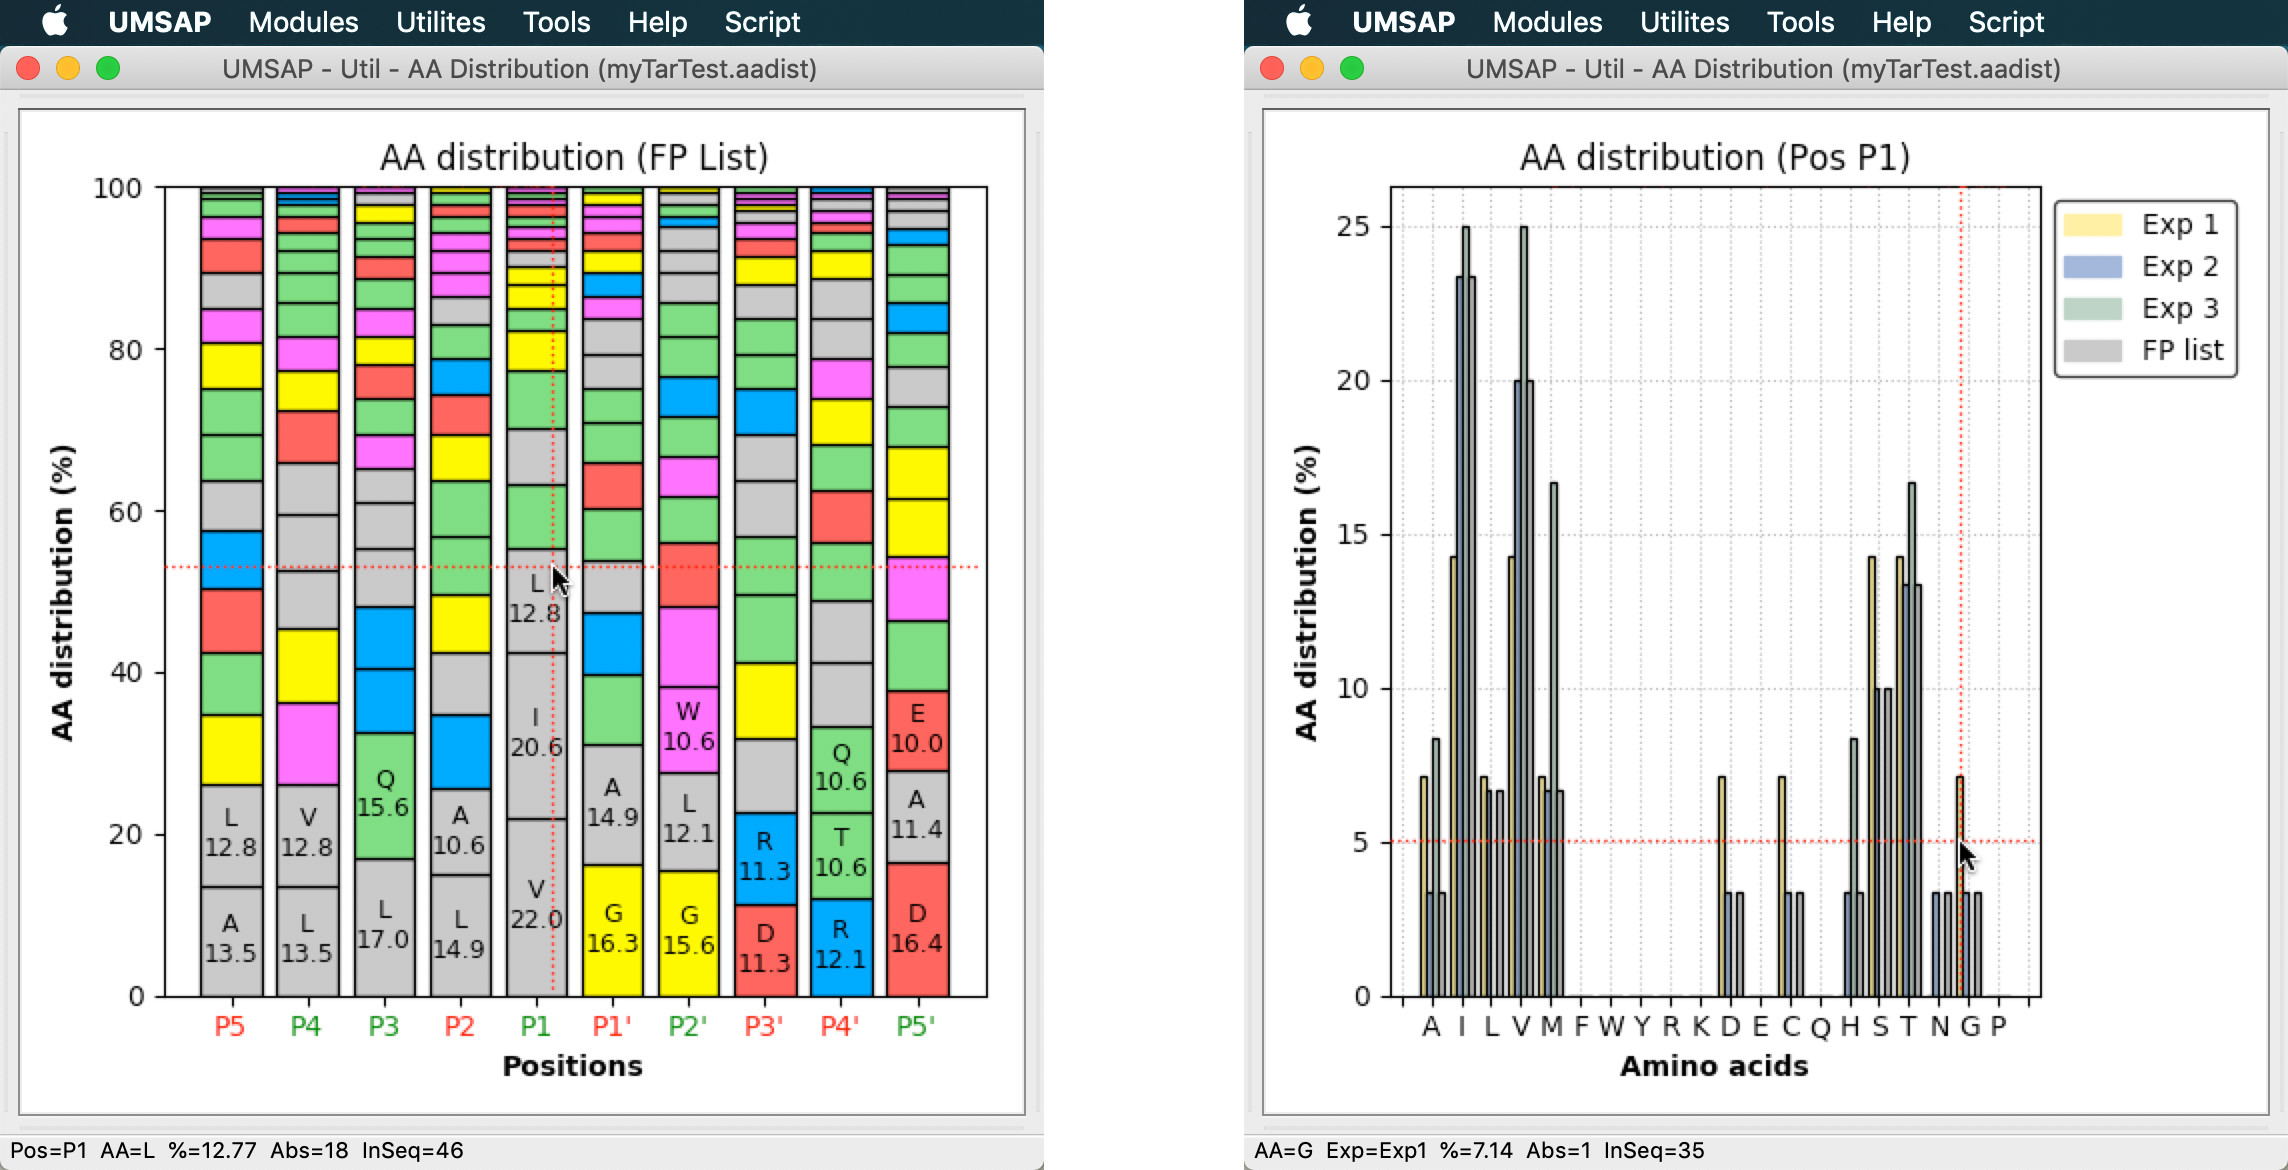
\includegraphics[width=0.9\textwidth]{./IMAGES/UTIL-AA-WINDOW/util-aa-res.jpg}	    
	\caption[The AA Distribution analysis window]{\textbf{The AA Distribution analysis window.} This window allows to visualize the results contained in a .aadist file.}
	\label{fig:utilAadistShow}
	\vspace{-5pt} 	
\end{figure}

\textit{\textbf{The output}} 

The output from the AA distribution calculation is a file with .aadist extension. The file will be automatically loaded and a graphical representation of the results will be shown (\autoref{fig:utilAadistShow}). There are two graphical representations. The first representation shows a bar graph of the AA distribution in which each bar represents a position. AAs are color coded with positively charged AAs (R and K) in blue, negatively charged AAs (D and E) in red, polar AAs (S, T, N, H, C and Q) in green, non-polar AAs (A, V, I, L and M) in gray, aromatic AAs (F, Y and W) in pink and Gly and Pro in yellow. AAs with an occurrence higher than \SI{10}{\percent} are labeled with the one letter code for the AA and the percentage value. For example, in \autoref{fig:utilAadistShow} the value of \SI{16.7}{\percent} obtained for A in position \(P1'\) means that A was found in position \(P1'\) in the \SI{16.7}{\percent} of the total cleavage sites detected. 

The results of the $\chi^2$ test are given in the color of the name of the position. A green color represents that the obtained distribution in the position is significantly different to a no selectivity distribution at the level of significance found in the .tarprot file. A red color represents that the distributions are not significantly different at the level of significance found in the .tarprot file. Finally, a black color indicates that the number of expected values below 5 was higher than the \SI{20}{\percent} threshold recommended by Yates et al. and the test was not performed \cite{Yates1999}. 

If the mouse pointer is placed on top of the bars, then information related to the bar and the AA will be shown in the status bar at the bottom of the window. The information includes the Position (Pos), the amino acid (AA), how many times does the AA appears in the position as a percent of the total AA count for the given position (\%) and the absolute number (Abs) and how many times does the AA appears in the sequence of the recombinant protein (InSeq).

The second representation allows to compare the AA distribution in one position across all experiments. This is also a bar representation in which each bar represents an experiment and each position an AA. Placing the mouse pointer over a bar shows information about it. The information includes the AA (AA), the experiment (Exp), how many times does the AA appears in the position for the given experiment as a percent of the total AA count found at the position for the given experiment (\%) and  the absolute number (Abs) and how many times does the AA appears in the sequence of the recombinant protein (InSeq).

\textit{\textbf{The Tools menu}}

By default, the AA distribution for all AA in the FP list will be shown when the .aadist file is loaded. The Tools menu in the window allows user to change the displayed experiment or to select the position for which results in the experiments should be compared. In addition, users may select to export the data shown in the window (see \autoref{subsec:utilExpData}), save a figure of the plot and to reset the view. 

\subsection{Cleavage Evolution}

\subsection{Cleavage Histograms}
\label{subsec:utilHistoCut}
The Histograms utility allows to create histograms of the identified cleavage sites using the residue numbers of the Target protein as the definition of the windows in the histograms. Histograms are created from a .tarprot file. How to generate the .tarprot file is discussed in \autoref{chap:tarprot}. Only FP are used to create the histograms, see page \pageref{par:tarprotPIP}. The list of FP is a non redundant list. 

\textit{\textbf{The interface}}

The Histograms window is divided in three regions (\autoref{fig:utilHistoCut}).

\begin{figure}[h]
	\centering
	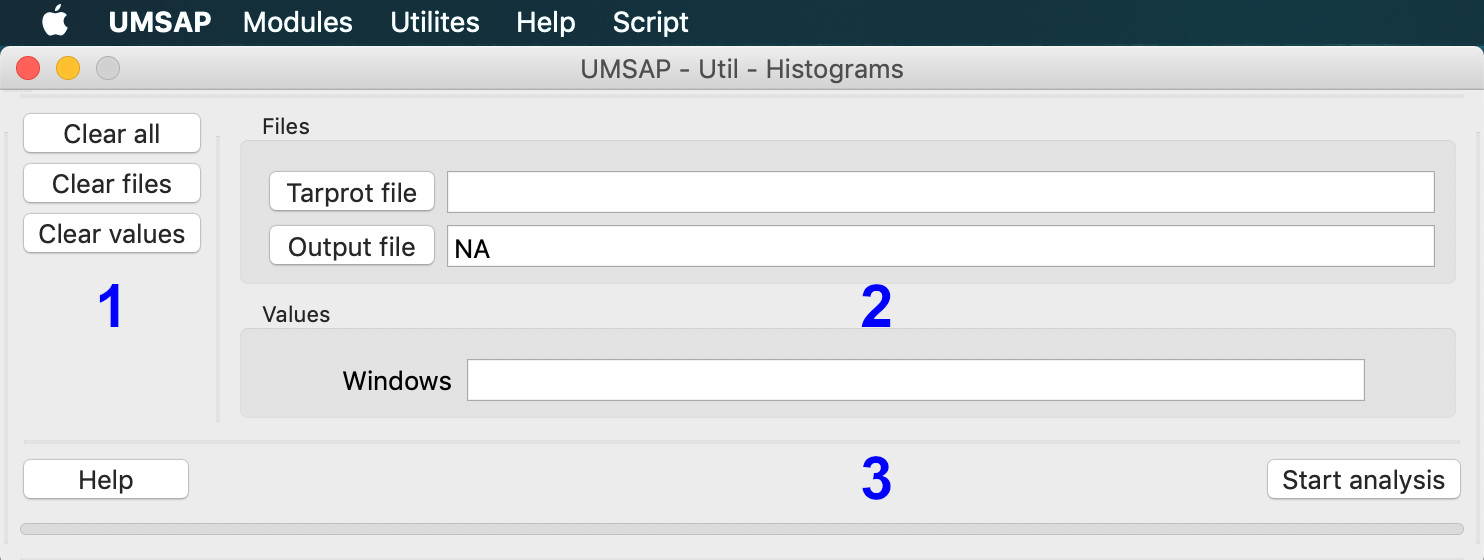
\includegraphics[width=0.9\textwidth]{./IMAGES/UTIL-HIST-WINDOW/util-histo.jpg}	    
	\caption[The Histograms utility window]{\textbf{The Histograms utility window.} This window allows to create histograms of the identified cleavage sites using the residue numbers of the Target protein as the definition of the windows in the histograms.} 
	\label{fig:utilHistoCut}
	\vspace{-5pt} 	
\end{figure}

Region \num{1} contains three buttons allowing users to quickly delete all provided input to generate a new .pdf file. The Clear all button will delete all user provided input. The Clear files button will delete all values in section Files of Region \num{2}. Finally, the Clear values button will delete all values in section Values of Region \num{2}.

Region \num{2} contains the fields where users provide the information needed in order to create the histograms. The Tarprot file button allows users to browse the file system to select the .tarprot file that will be used for the analysis. Only one .tarprot file can be selected here. The Output file button allows users to browse the file system to select the location of the .hist file to be created. If no Output file is selected the .hist file will be created in the same directory as the selected .tarprot file. If an older .hist file exists in the selected folder, UMSAP will append the date and time to the second to the end of the .hist file name in order to avoid overwriting the old .hist file. 

The parameter Windows allows to define the length of the windows in the histograms. Values here are expected to be integers greater than zero. A single value will results in equally spaced windows covering the entire length of the recombinant protein under study. Several values will result in custom sized windows. This may be useful if users want to define windows matching a structure related property of the Target protein e.g. secondary structure. In this case, the values must be space separated and organized from lower to higher values. For example, the input \numlist{1 50 100 200 220} will create four windows covering residues \numrange{1}{49}, \numrange{50}{99}, \numrange{100}{199} and \numrange{200}{219}.

Region \num{3} contains the Help and Start analysis buttons and a progress bar. The Help button leads to an online tutorial while the Start analysis button will start the analysis. The progress bar will give users a rough idea of the remaining processing time once the analysis is started.

\textit{\textbf{The analysis}}

First, UMSAP will check the validity of the user provided input. After this, the windows of the histograms will be created and for each experiment in the .tarprot file the detected cleavage sites will be assigned to the corresponding windows. Since most of the time the protein under study is a recombinant protein containing purification tags or only a region of the native protein, histograms are created for the residue numbers in the recombinant protein and for the residue numbers in the native protein. For this to be possible the sequence of the native protein must have been provided during the creation of the .tarprot file. In the last case cleavage sites outside the native sequence contained in the recombinant protein are discarded and the residue numbers used for the definition of the windows and cleavages sites are the residue numbers of the native sequence. After the analysis is done the .hist file will be automatically loaded and the results shown in a new window (\autoref{fig:utilHistoCutShow}).

\textit{\textbf{The output}}

The Histograms analysis window will display the results contained in a .hist file, see \autoref{fig:utilHistoCutShow}. In the histogram, experiments are shown in the order specified when creating the .tarprot file. In addition, the values for the histograms considering the results from all experiments (all FP) will be displayed as the last bar and colored in gray. Placing the mouse over the plot will display information at the bottom of the window. The information displayed includes the selected window (Win), the experiment represented by the bar (Exp) and the number of cleavages (Cleavages).

\begin{figure}[h]
	\centering
	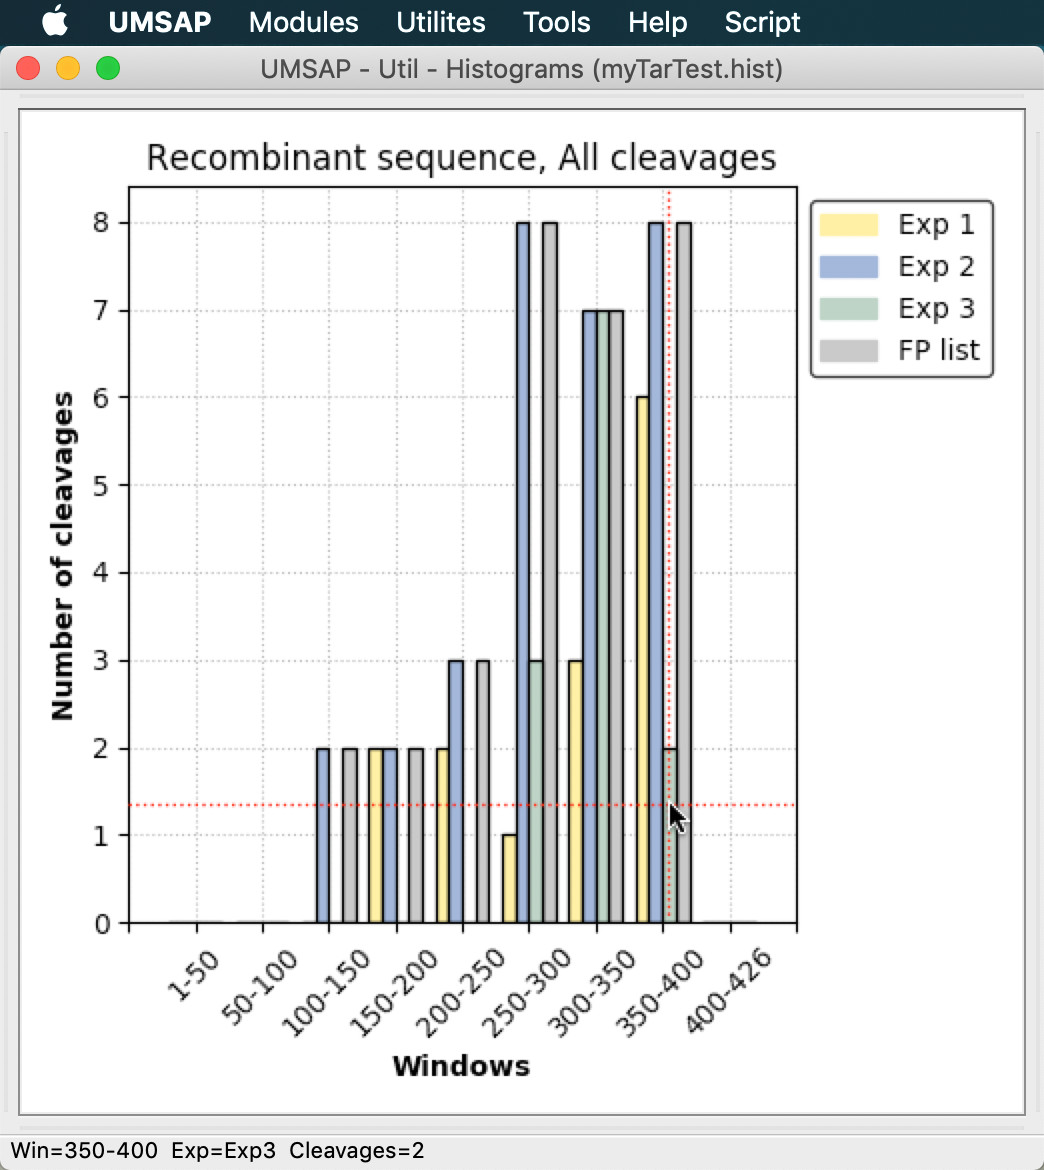
\includegraphics[width=0.7\textwidth]{./IMAGES/UTIL-HIST-WINDOW/util-histo-res.jpg}	    
	\caption[The Histograms analysis window]{\textbf{The Histograms analysis window.} This window allows to visualize the results contained in a .hist file.} 
	\label{fig:utilHistoCutShow}
	\vspace{-5pt} 	
\end{figure}

\textit{\textbf{The Tools menu}}

The Tools menu allows to show the results for the recombinant or native sequence and to show only unique cleavages or the total count of the detected cleavages. In addition, users may export the data shown in the window to a plain text file (see \autoref{subsec:utilExpData}), save an image of the plot or reset the state of the plot.

\subsection{Cleavage per Residue}
\label{subsec:utilCutsPerRes}
The Cleavages per residue utility calculates the absolute number of cleavages detected in the MS experiments for each residue in the recombinant protein under study. The peptides used to identify the cleavage sites are the FP contained in the .tarprot file used as input for the calculation (see page \pageref{par:tarprotPIP}). How to generate the .tarprot file is discussed in \autoref{chap:tarprot}. The FP list is a non redundant list.

\textit{\textbf{The interface}}

The Cleavages per residue utility does not have a window since there are no options to specify. When the utility is selected users will be asked to select a .tarprot file and then users must select the output file. That is all.

\textit{\textbf{The analysis}}

First, UMSAP will check the validity of the user provided input. After this the list of FP will be generated from the .tarprot file. Then, UMSAP will count how many times each residue in the protein under study appears at the C terminus of a FP or at the \(N-1\) position of a FP (\(N\) is the N terminus of the FP). The cleavages per residue value for the first and last residue of the protein under study is of course zero. This is done for every experiment in the .tarprot file and also taking into account the results for all experiments. Finally, UMSAP will take the absolute number of cleavages per residue and will normalize the values to bring them in the 0 to 1 range. Both the absolute and normalized values are written to the output file. After the analysis is done the results will be automatically loaded and displayed in a new window (\autoref{fig:utilCutsPerRes}). 

\textit{\textbf{The output}}

The output file from the Cleavages per residue utility will be shown as a simple number of cleavages vs residue number plot (\autoref{fig:utilCutsPerRes}). Residues with cleavages per residue higher than one third of the maximum number of cleavages per residue will be highlighted with an asterisk (*). Placing the mouse pointer inside the plot will display the residue number and the number of cleavages in the status bar at the bottom of the window. When two data sets are plotted simultaneously, the number of cleavages are given in the same order shown by the legend in the window. The gray vertical lines enclose the native residues. 

\textit{\textbf{The Tools menu}}

The window shows by default the absolute number of cleavages considering all FP for the recombinant protein. The Tools menu allows users to change this. Users may select to plot the results for a particular experiment or to compare two experiments. In addition, only the native sequence could be plotted or the normalized cleavages per residue values may be shown. An image of the plot can be created using the Save Plot Image entry in the Tools menu. The Reset View option restores the default appearance of the window. The Export Data option allows to save the data shown in the window to a plain text file.  

\begin{figure}[h]
	\centering
	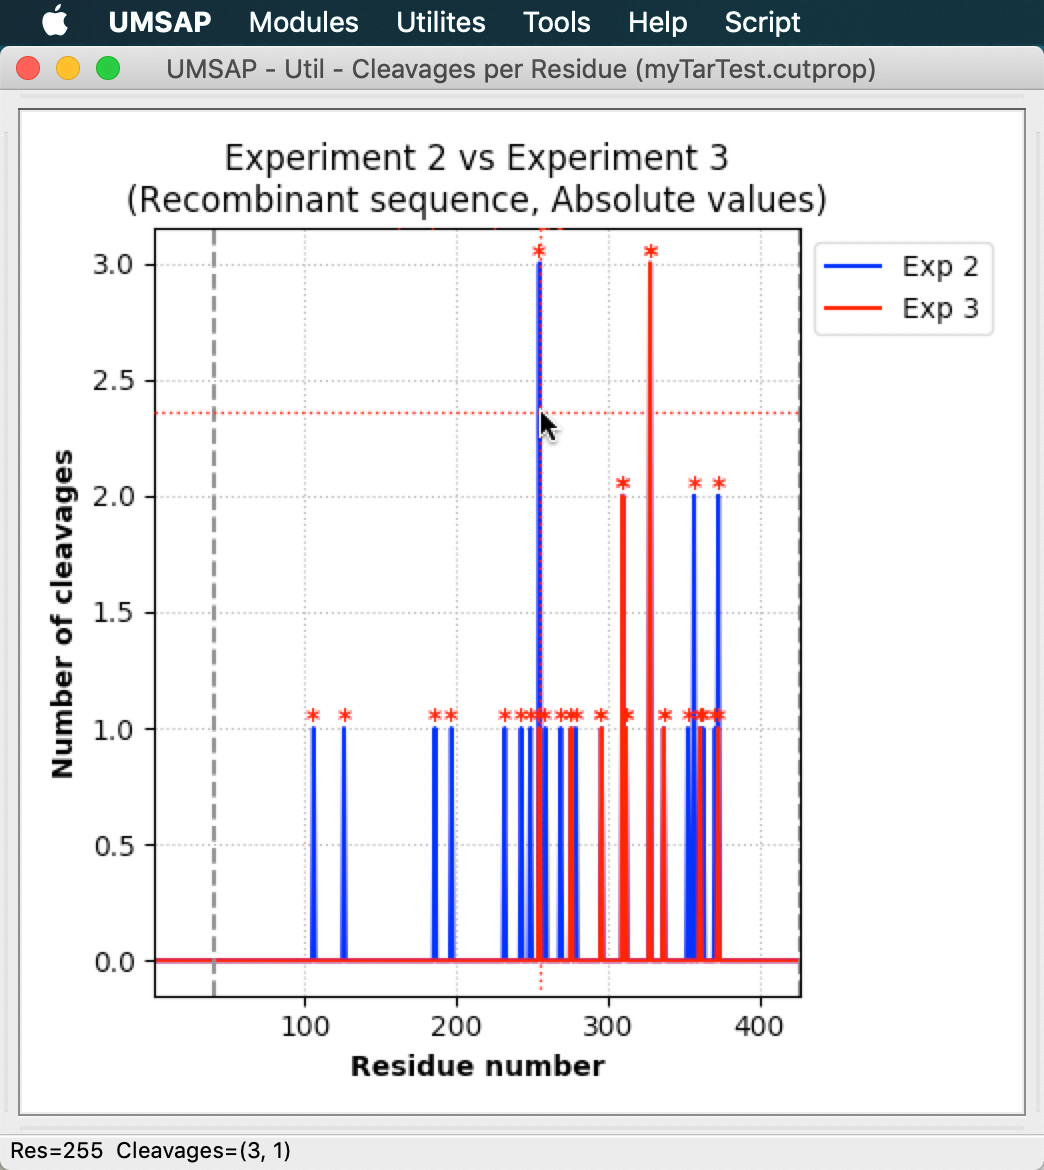
\includegraphics[width=0.7\textwidth]{./IMAGES/UTIL-CUTPROP-WINDOW/util-cutprop-res.jpg}	    
	\caption[The Cleavages per Residue analysis window]{\textbf{The Cleavages per Residue analysis window.} This window allows to visualize the results contained in a .cutprop file.} 
	\label{fig:utilCutsPerRes}
	\vspace{-5pt} 	
\end{figure}

\subsection{PDB Mapping}

\label{subsec:utilCut2Pdb}

The Cleavages to PDB Files utility maps the number of cleavages per residue found in a .tarprot file to a .pdb file containing the structure of the Target protein. The peptides used to identify the cleavage sites are the FP contained in the .tarprot file used as input for the calculation, see page \pageref{par:tarprotPIP}. How to generate the .tarprot file is discussed in \autoref{chap:tarprot}. The FP list is a non redundant list.

\textit{\textbf{The interface}}

The Cleavages to PDB Files window is divided in three regions, see \autoref{fig:utilCut2PDB}.

Region \num{1} contains three buttons allowing users to quickly delete all provided input to generate a new .pdf file. The Clear all button will delete all user provided input. The Clear files button will delete all values in section Files of Region \num{2}. Finally, the Clear values button will delete all values in section Values of Region \num{2}.

Region \num{2} contains the fields where users provide the information needed in order to perform the mapping of the number of cleavages. The Tarprot file button allows users to browse the file system to select the .tarprot file that will be use for the analysis. Only one .tarprot file can be provided here. The PDB file allows user to browse the file system to select a .pdb file. The .pdb file will contain the structure of the Target protein. This field can be left empty if the PDB file is to be downloaded from the PDB database. The Output folder button allows users to browse the file system to select the location of the resulting PDB folder containing the results. If left empty, then the PDB folder, resulting from the analysis, will be saved in the same directory containing the .tarprot file. If the Output folder option is left empty and the folder containing the selected .tarprot file already contains a PDB folder, then UMSAP will add the current date and time to the second to the end of the folder name in order to avoid overwriting the older PDB folder without explicit user permission.

The PDB ID field allows users to specify the chain or the segment id in the .pdb file that should be used for the mapping. Alternatively, if the PDB file field is left empty a code from the PDB database plus the chain or segment id may be given here. In this case, the pdb file will be directly downloaded from the PDB database. The expected syntax in this case is code;chain or code;segment for example, 2f4y;A or 2f4y;PROA.  

Region \num{3} contains the Help and Start analysis buttons and a progress bar. The Help button leads to an online tutorial while the Start analysis button will start the analysis. The progress bar will give users a rough idea of the remaining processing time once the analysis is started.

\begin{figure}[h]
	\centering
	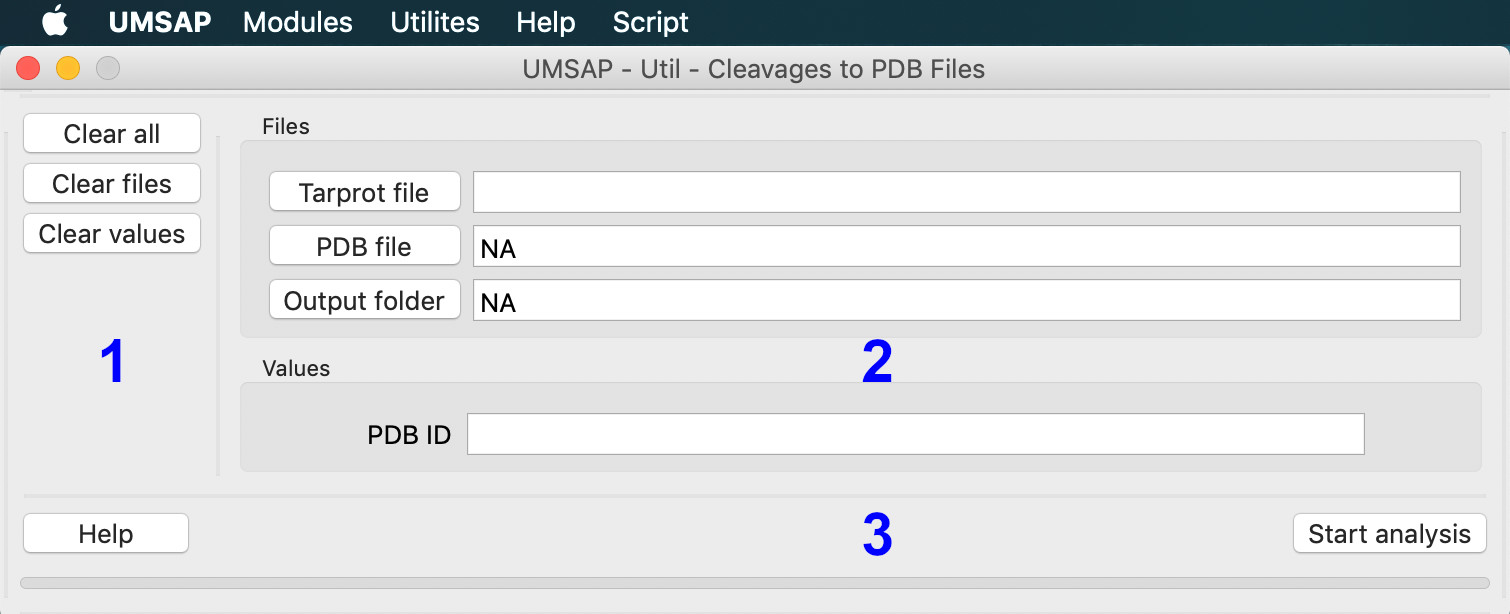
\includegraphics[width=0.7\textwidth]{./IMAGES/UTIL-PDB-WINDOW/util-pdb.jpg}	    
	\caption[The Cleavages to PDB Files utility window]{\textbf{The Cleavages to PDB Files utility window.} This window allows to map the detected number of cleavages per residue to a .pdb file containing the structure of the Target protein. The number of cleavages are mapped to the beta field in the .pdb.} 
	\label{fig:utilCut2PDB}
	\vspace{-5pt} 	
\end{figure}

\textit{\textbf{The analysis}}

First, UMSAP will check the validity of the user provided input. Then, a temporal .cutprop file will be created. Details about the .cutprop files can be found in \autoref{subsec:utilCutsPerRes}. After this, the sequence from the .pdb file is extracted and aligned with the sequence of the recombinant protein found in the .tarprot file. Finally, the number of cleavages found in the .cutprop file are mapped to the corresponding residues in the .pdb file.

\textit{\textbf{The output}}

The output from this utility is a series of .pdb files that will be saved in a PDB folder. Each file contains the number of cleavages mapped to the beta field of the corresponding residue in the .pdb structure. The results for each experiment and the FP list are mapped to individual files. The mapped values can be visualized by opening the .pdb files with VMD, PyMol or Chimera and coloring the structure by beta factors.




